\section{Elliptic curves}

\subsection{Elliptic curves' definition}

\begin{frame}[t]
    \frametitle{Elliptic curve}
    \begin{minipage}[t]{0.48\linewidth}
    \begin{definition}
        An elliptic curve define over a field $K$ is a projective plane curve where its
        homogeneous equation is
        \begin{align}
            \label{eq:ellipticCurve}
            y^2z = x^3 + axz^2 + b z^3
        ,\end{align}

        where $a$ and $b$ are elements of $K$ which verify the following condition
        \begin{align}
            \label{eq:delta}
        \Delta = - (4a^3 + 27 b^2) \neq 0
        .\end{align}
    \end{definition}
    \end{minipage}%
    \hfill%
    \begin{minipage}[t]{0.48\linewidth}
       \begin{figure}[h]
           \centering
           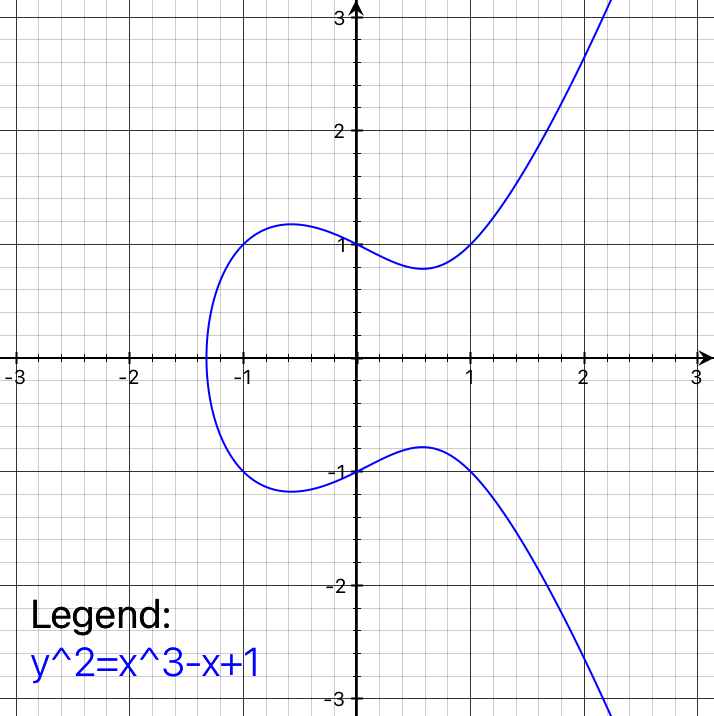
\includegraphics[width=0.8\textwidth]{courbeCanonique1}
           \caption{canonical curves with $\Delta < 0$}
           \label{fig:courbeCanonique1}
       \end{figure} 
    \end{minipage}
\end{frame}

\subsection{Rationals points}

\begin{frame}[t]
    \frametitle{Weierstrass normal equation and rationals points}
    \begin{minipage}[t]{0.48\linewidth}
        
    % \begin{alertblock}{}
       % As you can see on the figure \ref{fig:courbeCanonique1} and
       % \ref{fig:courbeCanonique2} we use the Weierstrass form which is
        \begin{itemize}
        \item \textbf{Weierstrass form}
       \[
       y^2=x^3+ax+b
       ,\] 
       % this way we have an elliptic curve $E$ define over a field $K$ equals to the following
       % set:
       \item \textbf{rationals points set}
       \[
    E(K) = \left\{ P \in \mathbb{P}_{2} \mid y^2 = x^3 + ax + b \right\} \cup \left\{
       \mathcal{O} \right\}  
       \] 
       \item \textbf{Infinity point}
       \[
       \mathcal{O} = [0,1,0]
       .\] 
        \end{itemize}
       % where $\mathcal{O}$ is the ideal point or infinity point of coordinates $[0,1,0]$.

       % The rationals points of an elliptic curves are the point of the projective plane
       % which are solution of \eqref{eq:ellipticCurve}.
    % \end{alertblock}
    \end{minipage}%
    \hfill%
    \begin{minipage}[t]{0.48\linewidth}
       \begin{figure}[h]
           \centering
           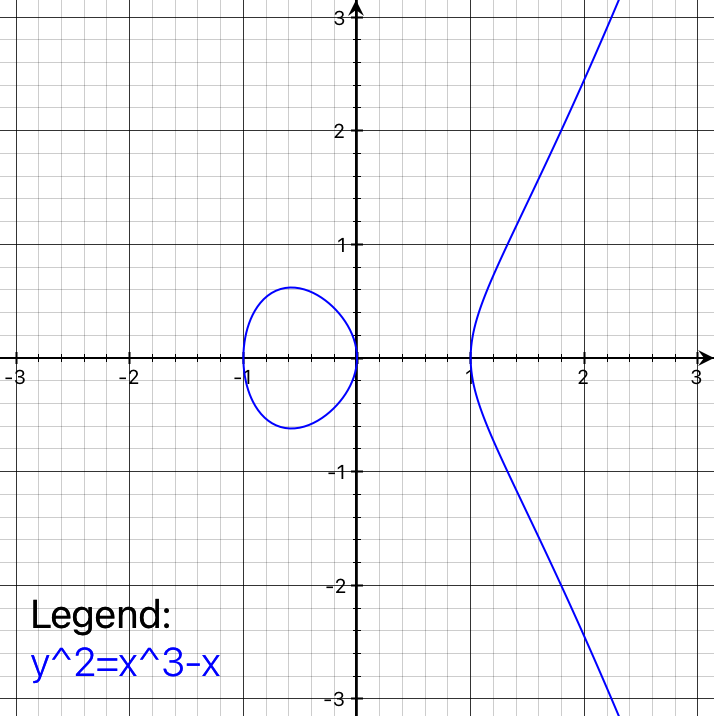
\includegraphics[width=0.8\textwidth]{courbeCanonique2}
           \caption{canonical curves with $\Delta > 0$}
           \label{fig:courbeCanonique2}
       \end{figure} 
    \end{minipage}
\end{frame}
